\documentclass[a4paper,11pt]{article}
%\usepackage{array}
%\usepackage{theorem}
\usepackage{graphicx}
\usepackage{fancyhdr}
\usepackage[toc,page]{appendix}
%\usepackage{times,mathptm}
%\usepackage[pdftex]{graphicx}
%\usepackage{color}
%\usepackage{caption}
%\usepackage{graphpap}
%\usepackage{rotating}
%\usepackage{epsfig}
%\usepackage{epsfig,psfrag}

%\setlength{\textwidth}{6.0in}
%\setlength{\textheight}{8.0in}
%\setlength{\topmargin}{0.in}
%\setlength{\headheight}{0.8in}
%\setlength{\headsep}{0.in}
%\setlength{\parindent}{0.25in}
%\setlength{\oddsidemargin}{0.2in}
%\setlength{\evensidemargin}{0.2in}

\newcommand{\ve}[1]{\mbox{\boldmath $ #1$}}
%opening
\title{TDStool: Notes on Numerical Methods}
\author{Andrea Bertoni, Thomas Serafini}



\begin{document}

%\setlength{\leftmargini}{\parindent} % Controls the indenting of the "bullets" in a list
%\pagestyle{empty}
%\pagenumbering{alph}
%\begin{minipage}[t][7.5in][s]{6.25in}
\begin{titlepage}

\flushright{
\Huge
TDS{\hspace{1mm}}tool}

\flushright{
\LARGE
\mbox{Time Dependent Schr{\"o}dinger equation simulation tool}}

\vspace{40mm}
\flushright{
\huge
\bf Notes on Numerical Methods}

\vspace{20mm}
\flushright{
\Large
Andrea Bertoni \\
\vspace{2mm}
Thomas Serafini}

\vspace{60mm}
\flushright{
\large
\today \\
Version 0.2 \\
TDStool Version 0.2}

\vspace{10mm}
\flushright{
\Large
S3 National Research Center, CNR-INFM \\ Modena, Italy}

\normalsize
%\vfill
% \flushright{\includegraphics[width=2.in]{FIGURES/nistident_flright_vec}}

\newpage

\pagestyle{empty}
\mbox{}
\end{titlepage}
%\end{minipage}
%\maketitle
%\begin{abstract}
%\end{abstract}

\section*{Preface}
The software TDStool is a numerical solver for the Time Dependent (linear)
Schr\"odinger equation and (nonlinear) Gross-Pitaevskii equation.
This document provides the theoretical basis for TDStool.
It describes the discretization methods and the main numerical
algorithms used in the code. It aims to be a technical reference guide
and a means to reach an in-depth understanding of the source code.
In fact, it should be the starting point for whoever is willing to
modify the code (released as an open-source project) and hopefully contribute
to the project.
Since the discussion in this note has been kept at a tutorial level, 
it can represent a nimble introduction to some of the numerical techniques
used in the code. However, we urge newcomers to read the references
suggested in the text.

\section*{Disclaimer}
We make no warranty to users of TDStool and accept no responsibility for
its use and for any conclusion drawn from its results.  Although we endeavour
to provide an easy-to-use software with an intuitive interface, TDStool is
primarily intended for use by those competent in the field of quantum mechanics
and numerical analysis.

\section*{Copyright}
At this early stage, the software TDStool and the related documentation
(including the present note) is copyrighted by the authors and their
employer.  The TDStool code is released as open-source and is free for
personal use.  We plan to release a later version of the software under
a public license.


\section*{About the Authors}
%(up-to-date as of \today)

{\bf Andrea Bertoni} %is
\\
{\bf Thomas Serafini} %is

\section*{Acknowledgements}
TDStool has been developed within the \emph{TDStool} INFM Seed project 2008.
We are pleased to thank Guido Goldoni (Universit\`a di Modena e Reggio Emilia)
and Massimo Rudan (Universit\`a di Bologna) for most helpful discussions and
suggestions.

\newpage

\tableofcontents

\newpage

\pagestyle{fancy}
\fancyhead[RO,RE]{TDStool: Notes on Numerical Methods}
\fancyhead[LO,LE]{ver. 0.2}


\section{Introduction}
The single-particle dynamics of a nonrelativistic quantum system follows
the so-called time-dependent Schr\"odinger equation (TDSE) that relates the time derivative
of the system state with the system Hamiltonian ${\cal H}$ and the state itself~\cite{messiahBOOK}.
In the real-space representation, for a spinless particle the TDSE is the partial differential equation 
\begin{equation} \label{tdse1}
i\hbar\frac{\partial}{\partial t}\psi({\bf r},t)= {\cal H} \psi({\bf r},t),
\end{equation}
where ${\bf r}$ is the position, $t$ the time coordinate, $\psi({\bf r},t)$ a complex-valued
function representing the quantum state, with $|\psi({\bf r},t)|^2$ the probability density in
${\bf r}$ and $t$.  The Hamiltonian ${\cal H}$ in the above
equation is a differential operator written in the real-space representation.

The aim of TDStool is to solve numerically Eq.~(\ref{tdse1}) once the initial condition
$\psi({\bf r},t=0)$ and a proper boundary condition on the computational domain are given.

We will first deal with a single particle moving in a static scalar (e.g. electric) potential,
then we will generalize the discussion to include time-dependent fields. 
The effect of a time-dependent
uniform magnetic field will be added in a future version of these notes.

For the sake of brevity, we will only consider 2D systems and domains, i.e. with ${\bf r}=(x,y)$.
Formulas for different dimensionality will be explicitly reported only if the generalization
is not straightforward. Where manifest, the spatial or time coordinates of the wave function and
operators will be implied.


\section{Schr\"{o}dinger equation with a scalar potential}

We consider a single particle subject to a potential $U(x,y,t)$, eventually dependent
on the time $t$.
We want to solve the TDSE Eq.~(\ref{tdse1}) on a rectangular domain
\begin{equation}
D = (x,y) \mid x\in[0,X], y\in[0,Y]
\end{equation}
with given $X$ and $Y$.
We assume Dirichlet conditions on the domain boundaries
\begin{equation}
\partial(D) = (0,y) \cup (X,y) \cup (x,0) \cup (x,Y) \mid x\in[0,X], y\in[0,Y]
\end{equation}
i.e. the values of the wave function $\psi(x,y,t)$ in the points $(x,y)\in\partial(D)$ are given.

The Hamiltonian of the system reads $ {\cal H} = - \frac{\hbar^2}{2m}\nabla^2 + U(x,y,t) $,
where $m$ is the mass of the particle.
Equation~(\ref{tdse1}) becomes the standard real-space TDSE for a single particle in a scalar
potential:
\begin{equation} \label{tdsestatic}
i\hbar \frac{\partial \psi}{\partial t} = - \frac{\hbar^2}{2m}\nabla^2 \psi(x,y,t)
+ U(x,y,t)\psi(x,y,t) .
\end{equation}


\section{Box Integration Method}

In order to discretize the spatial coordinates of the TDSE we employ
the Box Integration Method, also known as Finite Volume Method~\cite{eymardBOOK}.
We start by semidiscretizing the Schr\"{o}dinger equation in the space.
We work on the above special case where the domain $D$ is a box and we take
an orthogonal and separable discretization grid.
We are going to consider a 2D grid, but the discretization can easily be
extended to a higher dimensional domain.
Furthermore, for brevity we rewrite Eq.~(\ref{tdsestatic}) as
\begin{equation} \label{tdsenoconst}
\frac{\partial \psi}{\partial t} = -\beta \nabla G + v \, \psi \, ,
\end{equation}
where we have used the definitions
\begin{eqnarray}
\beta &=& i \frac{\hbar}{2m} , \\
v &=& \frac{1}{i \hbar} U , \\
G &=& \nabla \psi \, .
\end{eqnarray}

Let $ x_0 < x_1 < \cdots < x_{N+1} $ and $ y_0 < y_1 < \cdots < y_{M+1} $ be the coordinates of an
orthogonal grid, with $x_0=0$, $x_{N+1}=X$, $y_0=0$, $y_{M+1}=Y$.
The domain $D$ will be given by
\begin{equation}
D = [x_0, x_{N+1}] \times [y_0, y_{M+1}] \, .
\end{equation}
Note that we take a non-uniform but x-y separable discretization grid, as shown in Fig.~\ref{fig:bimgrid}. 

\begin{figure}
\centerline{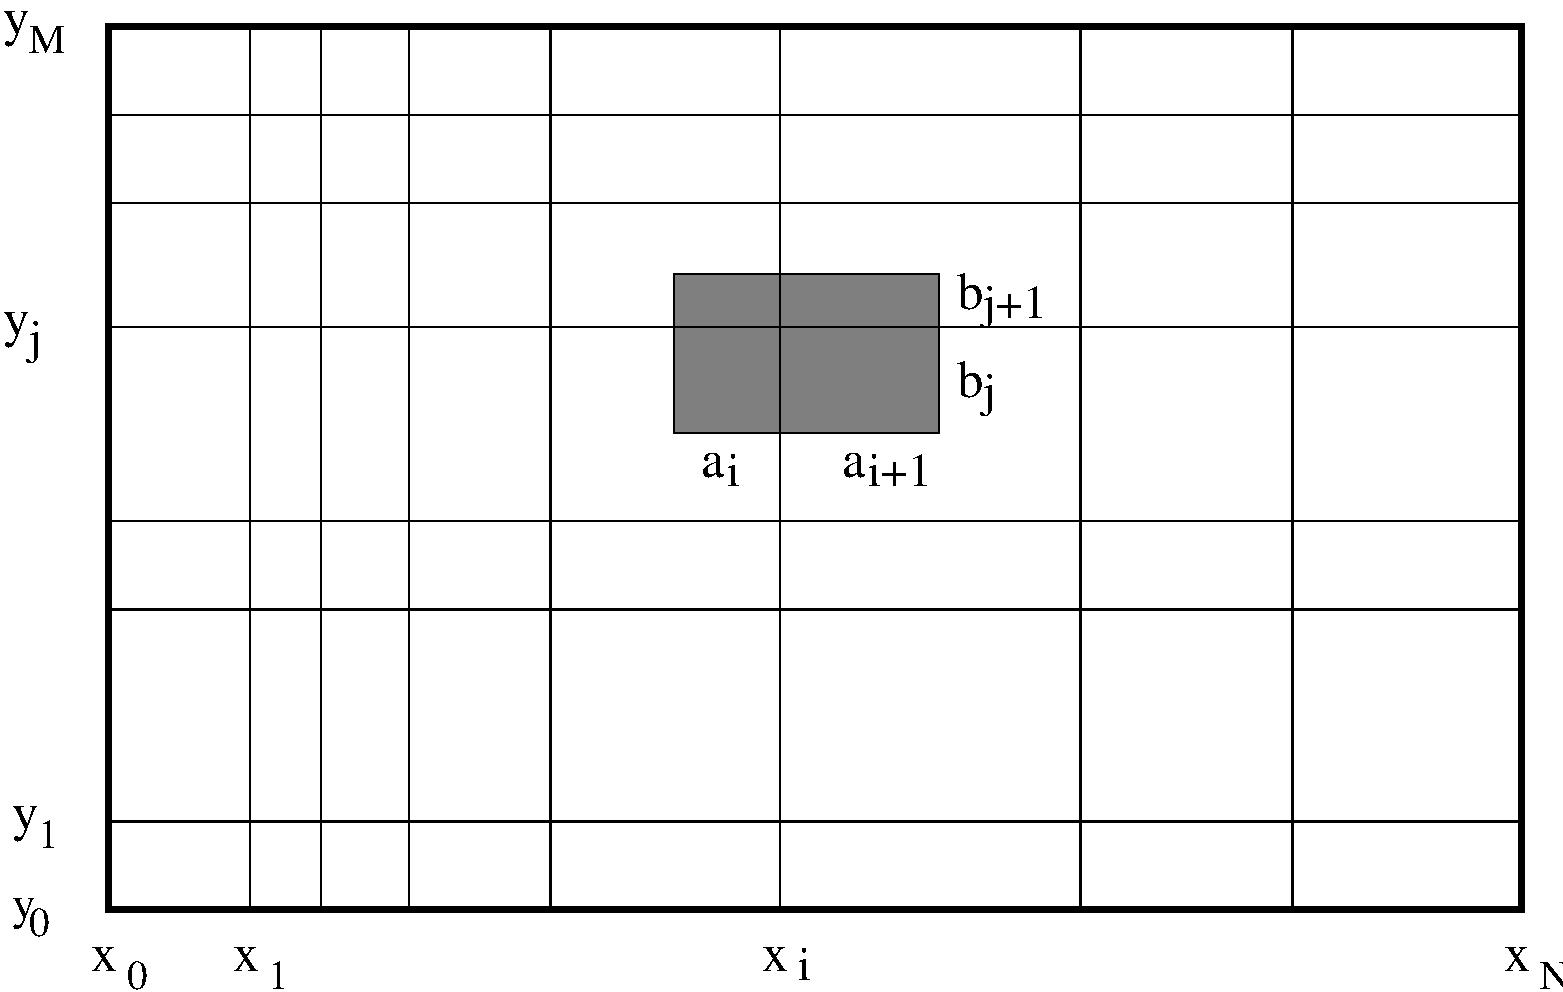
\includegraphics[width=2in] {bmgrid} }
\caption{Discretization grid on the 2D domain $D$.  The box $C_{ij}$ of area
$s_{ij}=\frac{a_i+a_{i+1}}{2} \frac{b_i+b_{i+1}}{2}$ is shaded.}
\label{fig:bimgrid}
\end{figure}

We will have $N \times M$ internal nodes in which the function $\psi$ is unknown.
The function $\psi(x, y, t)$ in the points where $x = x_0$ or $x = x_{N+1}$ or $y = y_0$ or $y = y_{M+1}$
is known thanks to the Dirichlet boundary conditions.

In order to solve the TDSE we use here a vertex-centred Box Integration Method.
First, we consider the internal grid points and partially cover the domain $D$
with $N \times M$ boxes 
\begin{equation}
C_{ij} = [\frac{x_i - x_{i-1}}{2}, \frac{y_j - y_{j-1}}{2}] \times
                [\frac{x_{i+1} - x_i}{2}, \frac{y_{j+1} - y_j}{2}] ,
\end{equation}
where $i = 1, \cdots, N$ and $j = 1, \cdots, M$.

If we call $a_i = x_i - x_{i-1}$ and
$b_j = y_j - y_{j-1}$, the area of the box $C_{ij}$ is
$s_{ij} = \frac{a_i+a_{i+1}}{2} \frac{b_i+b_{i+1}}{2}$.
Following the Box Integration Method we integrate Eq.~(\ref{tdsenoconst}) on each box $C_{ij}$:
\begin{equation}
\int_{C_{ij}} \frac{\partial \psi}{\partial t} \, ds = 
   \beta \int_{C_{ij}} \nabla G \, ds + 
   \int_{C_{ij}} v \, \psi \, ds \, .
\end{equation}

The three integrals can be approximated as follow:
\begin{eqnarray}
\int_{C_{ij}} \frac{\partial \psi}{\partial t} \, ds & \approx &
   s_{ij} \frac{d \psi}{dt}(x_i, y_j, t) \, , \\
\int_{C_{ij}} v \, \psi \, ds & \approx & s_{ij} (v \psi)(x_i, y_j, t) \, , \\
\int_{C_{ij}} \nabla G \, ds = \oint_{\partial C_{ij}} G \bar{\ve{n}} \, dl & \approx &
   (G_e \bar{\ve n}_e + G_n \bar{\ve n}_n + G_w \bar{\ve n}_w + G_s \bar{\ve n}_s) \, ,
   \label{green_int}
\end{eqnarray}
where the Green's theorem has been used in the latter expression.
$\bar{\ve n}_e$, $\bar{\ve n}_n$, $\bar{\ve n}_w$ and $\bar{\ve n}_s$ are the vectors normal to the four
edges of the box ${C_{ij}}$, and whose modulus is equal to the length of the edge (area of the surface in the 3D case);
$G_e$, $G_n$, $G_w$ and $G_s$ are the values of $G$, namely the gradient of $\psi$, in the mid point of each edge, as shown in Fig~\ref{fig:single_box}.

\begin{figure}
\centerline{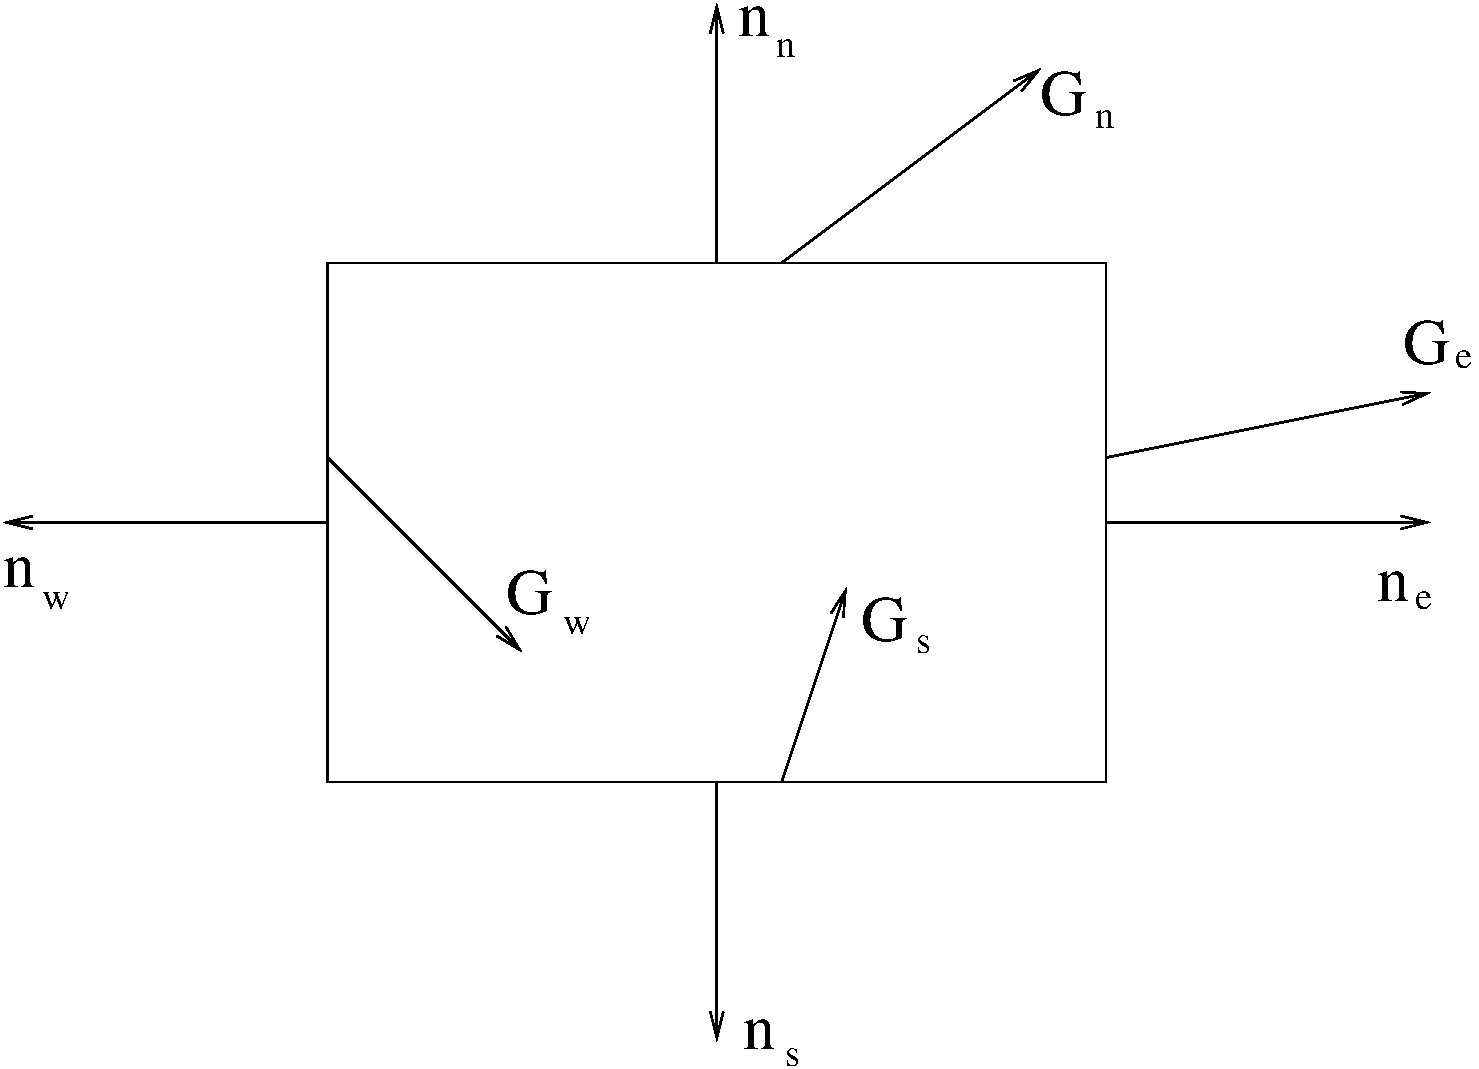
\includegraphics[width=2in] {box} }
\caption{Single box scheme}
\label{fig:single_box}
\end{figure}

Let define the space-discretized wave function $\psi_{i,j}(t) = \psi(x_i, y_i, t)$.
For ease of notation, here we use a two-index representation for $\psi_{ij}$ although this quantity is
represented in the code as a 1D array.  Specifically, $\psi_{i,j}$ means that we are referring to the element ${iM+j}$.
Using a centred difference formula, the gradient values $G$ can be approximated from the $\psi_{i,j}$ values on the nodes: 
\begin{eqnarray}
G_e \bar{\ve n}_e & \approx & \frac{\psi_{i,j}-\psi_{i-1,j}}{a_i} \frac{b_j+b_{j+1}}{2} \, ,      \\ \nonumber
G_n \bar{\ve n}_n & \approx & \frac{\psi_{i,j}-\psi_{i+1,j}}{a_{i+1}} \frac{b_j+b_{j+1}}{2} \, ,  \\ \nonumber
G_w \bar{\ve n}_w & \approx & \frac{\psi_{i,j}-\psi_{i,j-1}}{b_j} \frac{a_i+a_{i+1}}{2} \, ,      \\ \nonumber
G_s \bar{\ve n}_s & \approx & \frac{\psi_{i,j}-\psi_{i,j+1}}{b_{j+1}} \frac{a_i+a_{i+1}}{2} \, .     \nonumber
\end{eqnarray}

Let us now define
\begin{eqnarray}
k_1 &=& \frac{b_j+b_{j+1}}{2a_i}, \qquad k_2 = \frac{b_j+b_{j+1}}{2a_{i+1}}  \, ,      \\ \nonumber
k_3 &=& \frac{a_i+a_{i+1}}{2b_j}, \qquad k_4 = \frac{a_i+a_{i+1}}{2b_{j+1}}  \, .     \nonumber
\end{eqnarray}

The approximation of the integral in Eq.~(\ref{green_int}) becomes
\begin{eqnarray}
\lefteqn{\int_{C_{ij}} \nabla G \, ds \approx}   \\ \nonumber
& \approx &   (k_1+k_2+k_3+k_4) \, \psi_{i, j} + 
k_1 \, \psi_{i-1,j} + k_2 \, \psi_{i+1,j} + k_3 \, \psi_{i,j-1} + k_4 \, \psi_{i,j+1} \, .
\end{eqnarray}

If a box is adjacent to the boundary of the domain, some of the $\psi_{i,j}$ terms of the summation are defined by the boundary conditions rather than being unknown.  In this case we can group all these terms in one constant term.
For example, if $(i, j) = (1, 1)$, then $\psi_{i-1,j}$ and $\psi_{i,j-1}$ are on the boundaries and the above expression becomes
\begin{eqnarray}
\lefteqn{\int_{C_{11}} \nabla G \, ds \approx}   \\ \nonumber
& \approx &   (k_1+k_2+k_3+k_4) \, \psi_{1,1} + 
k_2 \, \psi_{2,1} + k_4 \, \psi_{1,2} + d_{11} \, .
\end{eqnarray}
where $d_{11} = k_1 \, \psi_{0,1} + k_3 \, \psi_{1,0}$ is the constant term that includes the known
values of $\psi$ at the boundaries.

In vector form, for each given box $C_{ij}$ these summations can be represented as a scalar product:
\begin{equation}
\ve m_{ij} \ve \psi + d_{ij} = \sum_{(k,l)=(1,1)}^{(N,M)} m_{ij}^{k,l} \, \psi_{k,l} + d_{ij}
\end{equation}
with $\ve \psi$ representing the column vector of the wave function and
with $\ve m_{ij} \in R^{N \times M}$ defined by
\begin{eqnarray}
\lefteqn{ \ve m_{ij} = (m_{ij}^{1,1}, m_{ij}^{1,2},\cdots, m_{ij}^{N,M}) = }  \\ \nonumber
&=&(0,\cdots, 0, \, k_1, 0, \cdots, 0, \, k_3, k_1+k_2+k_3+k_4, k_4 \, , 0,\cdots, 0, \, k_2, 0, \cdots, 0) \, .
\end{eqnarray}
Thus, the Schr\"{o}dinger equation can be approximately integrated on the box $C_{ij}$ with
\begin{equation}
s_{ij} \frac{d \psi_{i,j}}{dt}(t) = 
\beta \ve m_{ij} \ve \psi(t) + s_{ij} \, v_{ij} \, \psi_{i,j}(t) + \beta d_{ij} \, ,
\end{equation}
where $v_{ij}=v(x_i,x_j)$. 

By defining the diagonal matrices $S = \mbox{diag}(s_{ij})$ and $V = \mbox{diag}(v_{ij})$,
and the matrix whose columns are the vectors $\ve m_{ij}$: $M = \beta [\ve m_{ij}]$,
the equation can be written in matrix form:
\begin{equation} \label{tdsematrixform}
S \frac{d \ve \psi}{dt}(t) = M \ve \psi(t) + S V \ve \psi + \beta \ve d \, ,
\end{equation}
where the vector symbol $\ve d$ represents the column vector
$\ve d = (d_{11}, d_{12},\cdots, d_{NM})$, as usual.

For the \emph{time discretization} we use a Cranck-Nicholson scheme (also known as
trapezoidal rule).  By considering a time step $\Delta_t$, Eq.~(\ref{tdsematrixform}) becomes:
\begin{equation}
S {\ve \psi}(t+\Delta_t) = S \ve \psi(t) + \frac{(M+SV)\Delta_t}{2} 
\left( \ve \psi(t) + \ve \psi(t+\Delta_t) \right) + \beta \Delta_t \ve d
\end{equation}
or equivalently
\begin{equation} \label{CNmatrix}
\left( S - \frac{(M+SV)\Delta_t}{2} \right) \ve \psi(t+\Delta_t) =
\left( S + \frac{(M+SV)\Delta_t}{2} \right) \ve \psi(t) + \beta \Delta_t \ve d
\end{equation}

Note that in case the potential $v$ is dependent on the time, the two matrices $V$ on
the left and right sides of Eq.~(\ref{CNmatrix}) must be computed at the later and earlier
time step, respectively.
By making explicit the above equation for $\psi(t+\Delta_t)$ one gets
\begin{equation}
\ve \psi(t+\Delta_t) =
\frac{ 2\beta \Delta_t \ve d \ + \ \left(2S + \left( M+S\,V(t) \right)\Delta_t\right) \ve \psi(t) }
{2S - \left( M+S\,V(t+\Delta_t)\right)\Delta_t}
\end{equation}


\section{Gross-Pitaevskii equation}

The time-dependent Gross-Pitaevskii equation describes the collective coherent dynamics of
an ensemble of quantum particles, interacting through a Hartree pseudopotential.
This approximation results in an additional potential-like term in the time-dependent
Scr\"{o}dinger equation, proportional to the local particle density $|\psi({\bf r})|^2$.
In fact, the Gross-Pitaevskii model leads to the following nonlinear form of the
Schr\"odinger equation~\cite{leggettRMP01}
\begin{equation} \label{gpeq}
i \hbar \frac{\partial}{\partial t} \psi =
   -\frac{\hbar^2}{2m} \nabla^2 \psi(x,y,t) +
   \left(U(x,y,t) + \frac{4 \pi \hbar^2 a_s}{m} |\psi(x,y,t)|^2 \right) \psi(x,y,t) \, ,
\end{equation}
where $U$ is an external potential, as in the linear case, and $a_s$ is the
particle-particle scattering length. 

In this case, we suppose periodic boundary conditions on the domain $D$.
We rewrite Eq.~(\ref{gpeq}) highlighting the linear part and the nonlinear part of the operator,
$\cal L$ and $\cal N$, respectively:
\begin{equation}
\frac{\partial}{\partial t} \psi = {\cal L} \psi + {\cal N} \psi \label{eq:splitop}
%\psi(x, 0) & = & \psi_0(x) \, ,
\end{equation}
with
\begin{equation} \label{LandN}
{\cal L} = \frac{i\hbar}{2m} \nabla^2 \ \qquad \mbox{and} \qquad
{\cal N} = -i \left(\frac{1}{\hbar}U + \frac{4 \pi \hbar a_s}{m} |\psi|^2 \right) \, .
\end{equation}

The evolution of the wave function can be obtained through the evolution
operator ${\cal U}$
\begin{equation} \label{ssUoperator}
\psi(t+dt) = {\cal U}(t,t+dt) \, \psi(t) = {\cal T}\exp\left( \int_t^{t+dt}
({\cal L} + {\cal N}(t')) \, dt' \right) \, \psi(t) \, ,
\end{equation}
where ${\cal T}$ is the time-ordering operator and the time dependence of ${\cal N}$
has been explicitated.

Note that, if the operator ${\cal N}$ did not depend on the time, the
evolution operator would be ${\cal U}(t,t+dt) = e^{\left({\cal L} + {\cal N} \right) dt}$.
However, in the following we do not impose such a condition.


\section{Split-step Fourier Method}

In order to compute numerically the evolution of the wave function, we use a second-order
approximation formula to decompose the evolution operator ${\cal U}$.

In fact, we suppose that the operator ${\cal N}$, containing the
time-dependent potential and the particle density, varies slowly with the time.
Thus, a suitable $n$-th order decomposition formula for the time-ordered exponential
can be used\cite{suzukiPJA93,weidemanSIAM86}, with a negligible error of the order $O(dt^{n+1})$

The first-order approximate decomposition of ${\cal U}$ reads:
\begin{equation}
{\cal U}(t,t+dt) \approx e^{{\cal L}dt} e^{{\cal N}(t+\frac{dt}{2})dt} + O(dt^2) \, ,
\end{equation}
while the second-order decomposition reads:
\begin{equation}
{\cal U}(t,t+dt) \approx e^{\frac{1}{2}{\cal N}(t+\frac{dt}{2})dt}
e^{{\cal L}dt} e^{\frac{1}{2}{\cal N}(t+\frac{dt}{2})dt} + O(dt^3) \, ,
\end{equation}

%Fourth order approximation:
%$$ A_4(dt) = A_2(wdt) A_2((1-2w)dt) A_2(wdt) \, \quad
%   w = \frac{2+\sqrt[3]{2} + \frac{1}{\sqrt[3]{2}}}{3} $$

It is easy to see that the wave function evolution obtained
with the above first-order approximation,
$\psi(t+dt) = e^{{\cal L}dt}e^{{\cal N}(t+\frac{dt}{2})dt}\psi(t)$
is equivalent to perform two subsequent $dt$ steps through the equations
\begin{equation} \label{NLpde}
\frac{\partial}{\partial t} \psi = {\cal N}\left(t+\frac{dt}{2}\right) \psi
\qquad \mbox{and} \qquad
\frac{\partial}{\partial t} \psi = {\cal L} \psi \, .
\end{equation}

Similarly, the second-order evolution is equivalent to first perform
a step of $\frac{dt}{2}$ with the nonlinear operator ${\cal N}$ at time $t+\frac{dt}{2}$,
then a $dt$ step with
$\cal L$, finally another $\frac{dt}{2}$ step with ${\cal N}(t+\frac{dt}{2})$.
Now, the problem comes down to compute the separate evolutions generated by ${\cal N}$ and ${\cal L}$.

From Eq.~(\ref{LandN}), it is clear that the operator ${\cal N}$ is diagonal
in the real-space representation. Thus, its effect is local on each point
of the wave function:
\begin{equation}
{\cal N}\left(t+\frac{dt}{2}\right) \, \psi(x, y, t) =
e^{-i \left(\frac{1}{\hbar}V(x,y) + \frac{4 \pi \hbar a_s}{m} |\psi(x,y,t)|^2 \right) dt} \,
\psi(x, y, t) 
\end{equation}

On the other hand, the eigenvectors of the operator $i\hbar{\cal L}$ are known
analytically since they are the set of plane waves $e^{i {\bf k}\cdot{\bf r}}$.
The linear evolution of $\psi$
%(apart from the constant $i\hbar$)
can be obtained easily on the reciprocal $k$ space.
In order to do so, the wave function must be Fourier transformed. Then, the
linear evolution can be applied directly since its effect is local in $k$ space.

Starting from $\psi(x,y,t)$, the steps are the following:
\begin{eqnarray}
 \bar{\psi}(k_x,k_y,t) &=& \mathsf{FFT}[\psi(x,y,t)] \\
 \bar{\psi}(k_x,k_y,t+dt) &=& \bar{\psi}(k_x,k_y,t)
 e^{\frac{i\hbar}{2m} (k_x^2+k_y^2)dt} \label{klinearevolution} \\
 \psi(x,y,t+dt) &=& \mathsf{IFFT}[\bar{\psi}(k_x,k_y,t+dt)] \, ,
\end{eqnarray}
where $\mathsf{FFT}$ and $\mathsf{IFFT}$ indicate the Fourier transform and inverse Fourier transform,
respectively. A Fast Fourier Transform algorithm is used to compute the above transformations.

Let $ x_0 < x_1 < \cdots < x_{N+1} $ and $ y_0 < y_1 < \cdots < y_{M+1} $ be the coordinates of a
\emph{uniform} orthogonal grid, with $x_0=0$, $x_{N+1}=X$, $y_0=0$, $y_{M+1}=Y$.
It is important to properly define the frequency components on the corresponding $k$ grid.
In fact, if a wave function is defined on $[0, X]\times[0,Y]$ and
the $x$ axis is discrtized on $N+2$ points,
the $(k_x)_i$ are defined as:
\begin{equation}
(k_x)_i = \left\{ 
         \begin{array}{rll}
         &\frac{2 \pi (i-1)}{X} & i = 1, \ldots, \frac{N + 2}{2} \\
         -&\frac{2 \pi (N+3-i)}{X} & i = \frac{N+2}{2}+1, \ldots, (N + 2) \\
         \end{array} \right. \; .
\end{equation}

\newpage

\begin{appendices}
\section{Notation}

The following notation will be used for the spatial derivatives of a complex functional
$f:(x_1,\cdots, x_n)\mapsto C$:
\begin{eqnarray}
\nabla f &=& \mbox{grad}(f) =
\left( \frac{\partial f}{\partial x_1}, \cdots, \frac{\partial f}{\partial x_n} \right) \\
\nabla \cdot f &=& div(f) = \frac{\partial f}{\partial x_1} + \cdots + \frac{\partial f}{\partial x_n} \\
\nabla^2 f &=& \nabla \cdot \nabla f =
    \frac{\partial^2 f}{\partial x_1^2} + \cdots + \frac{\partial^2 f}{\partial x_n^2}
\end{eqnarray}

\end{appendices}

\begin{thebibliography}{5}

\bibitem{messiahBOOK}
A. Messiah, \emph{Quantum Mechanics} (vol. 1), North Holland, J. Wiley \& Sons, 1966.

\bibitem{eymardBOOK}
R. Eymard, T. Gallou\"et, R. Herbin, The Finite Volume Method, in \emph{Handbook for Numerical Analysis},
Ph. Ciarlet, J. L. Lions eds., North Holland, 2000.

\bibitem{leggettRMP01}
A. J. Leggett, Bose-Einstein condensation in the alkali gases: Some fundamental concepts,
Rev. Mod. Phys.~\textbf{73}, 307 (2001).

\bibitem{suzukiPJAB93}
M. Suzuki, General decomposition theory of ordered exponentials,
Proc. Japan Acad. ser. B~\textbf{69} 161, (1993).


\bibitem{weidemanSIAM86}
J.A.C. Weideman, B. M. Herbst, Split-step methods for the solution of the nonlinear
Schr\"odinger equation, SIAM J. Numer. Anal. \textbf{23}, 485 (1986).

%\bibitem{xuJMMA03}
%X. Xu, T. Taha, Parallel split-step fourier methods for nonlinear schroedinger-type equations,
%J. Math Model. Algo. \textbf{2}, 185 (2003).

\end{thebibliography}

\section*{See also}

\begin{trivlist}
\item
X. Xu, T. Taha, Parallel split-step fourier methods for nonlinear Schr\"odinger-type equations,
J. Math Model. Algo. \textbf{2}, 185 (2003).
\item
B. I. Schneider, L. A. Collins and S. X. Hu,
Parallel solver for the time-dependent linear and nonlinear Schr\"odinger equation,
Phys. Rev. E \textbf{73}, 036708 (2006).
\item
N. Watanabe and M. Tsukada,
Fast and stable method for simulating quantum electron dynamics,
Phys. Rev. E \textbf{62}, 2914 (2000).
\item
S. Blanes and P. C. Moan,
Splittings methods for the time-dependent Schr\"odinger equation,
Phys. Lett. A \textbf{265}, 35 (2000).
\item
R. Sch\"afer and R. Blendowske,
On the numerical solution of the time-dependent
Schr\"odinger equation,
J. Comp. Phys. \textbf{119}, 206 (1995).
\end{trivlist}

\end{document}
